
\begin{frame}{My Contribution towards issues/challenges}
  \begin{figure}
    \centering
    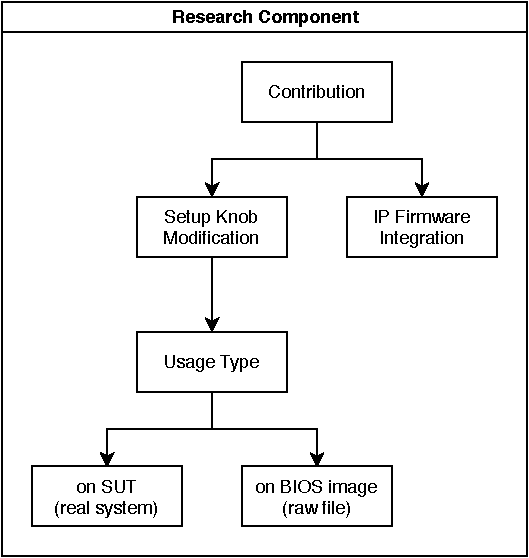
\includegraphics[width=\textwidth]{Im/figures/research-component}
%    \caption{Research Component}
%    \label{fig:research-component}
  \end{figure}
\end{frame}

% ========================================================================
% MODULE 1
% ========================================================================
\subsection{Setup Knobs Modification}
\begin{frame}[allowframebreaks]{Setup Knobs Modification: Process Flow}
  \begin{figure}[htbp]
    \centering
    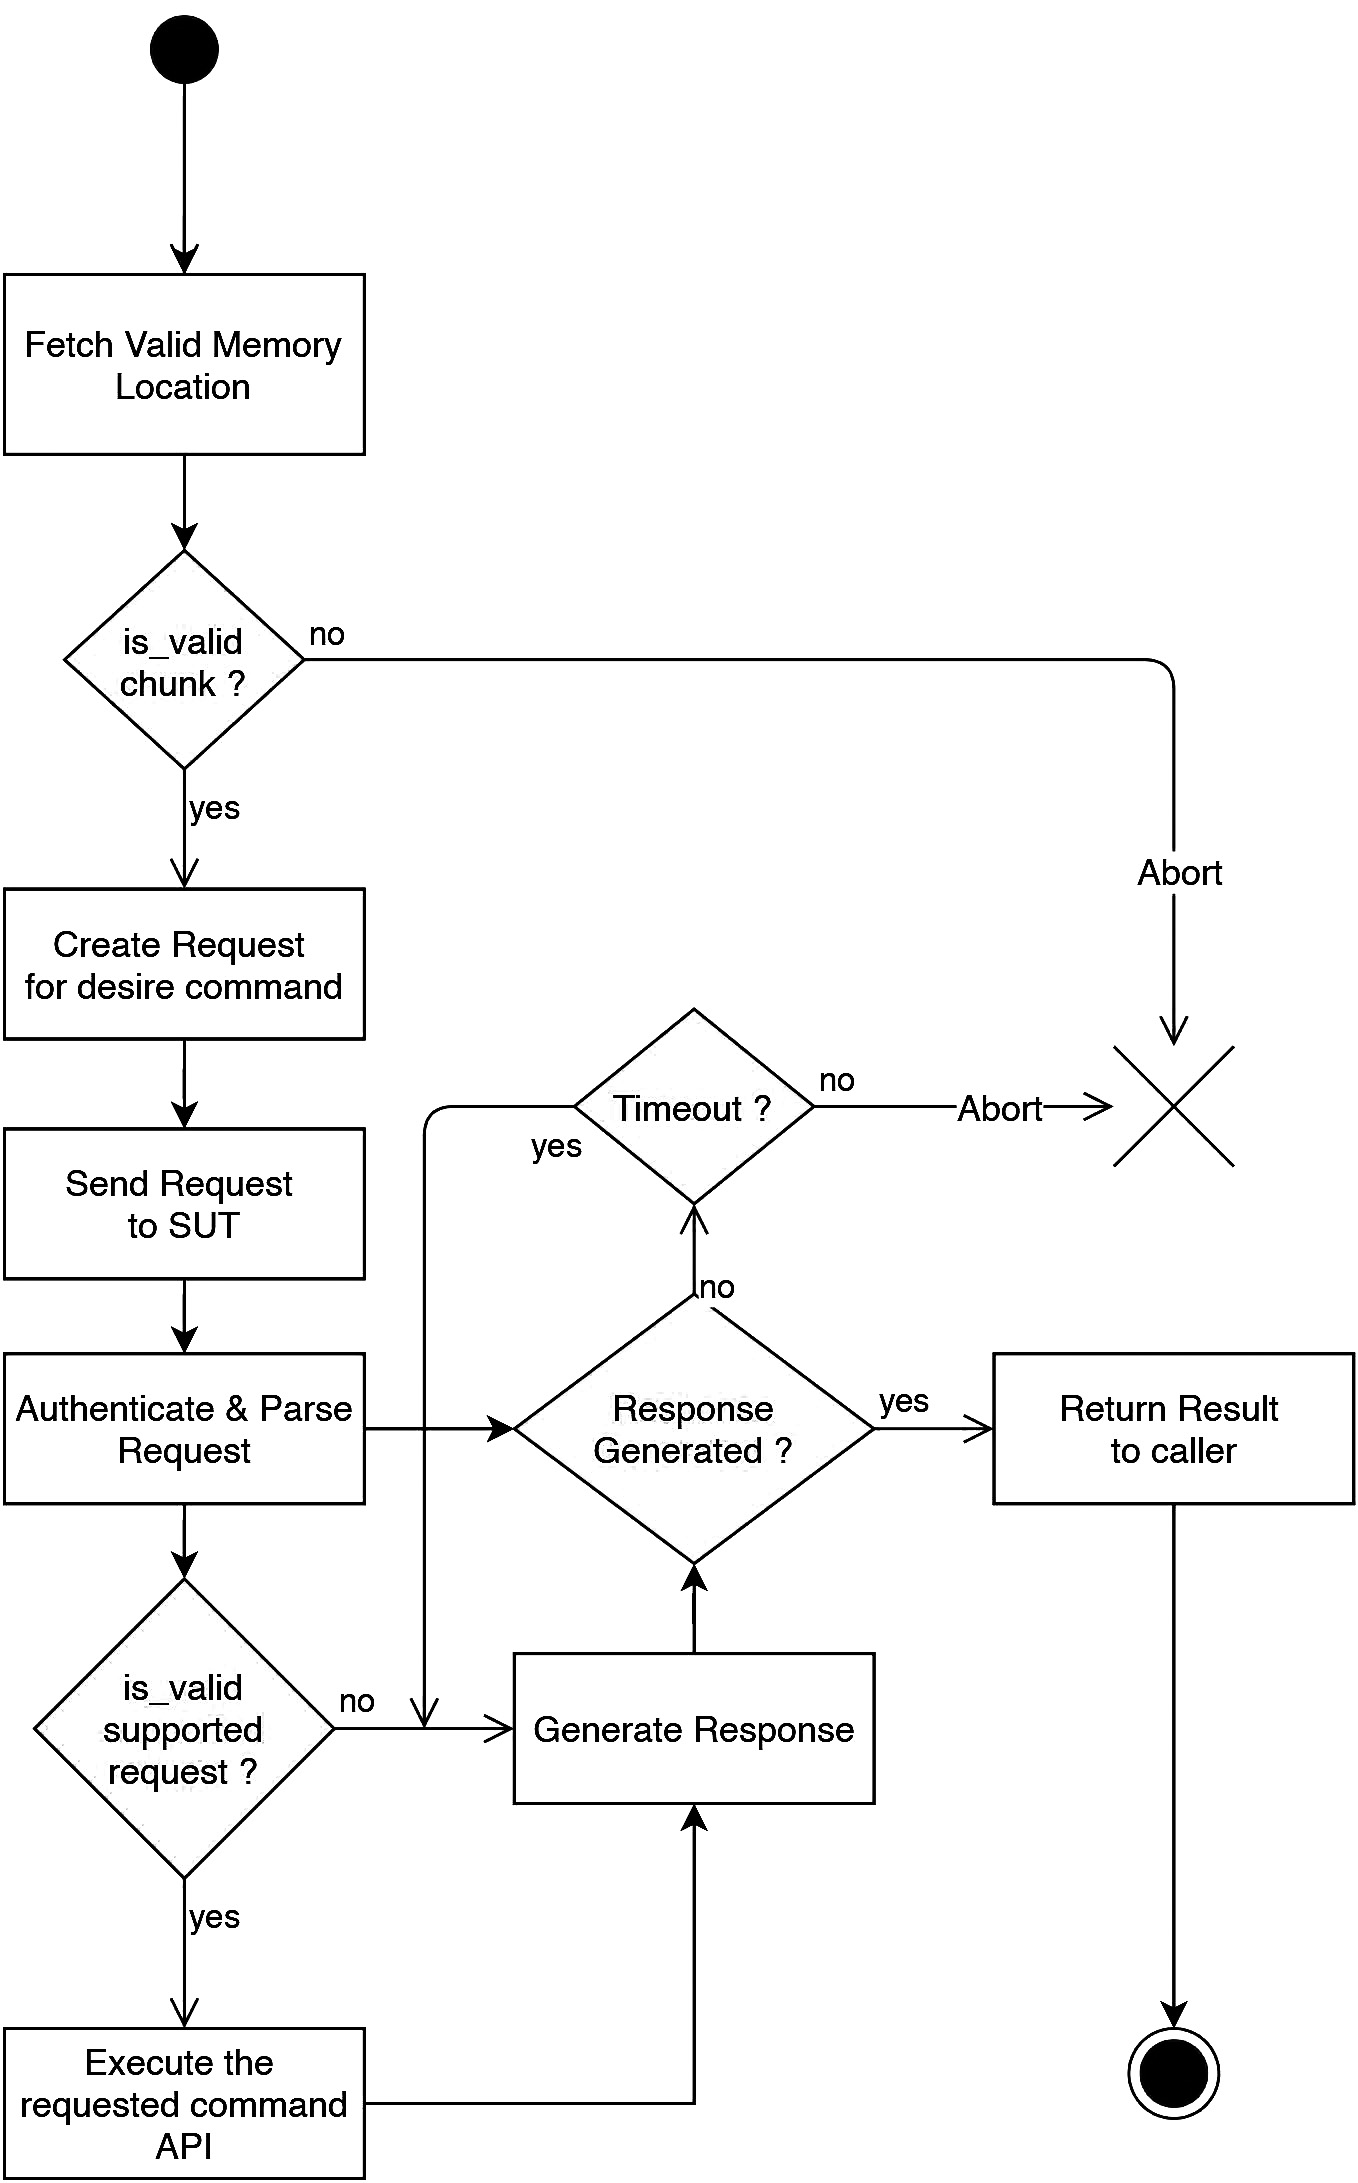
\includegraphics[width=0.3\linewidth]{Im/figures/setup-knobs-flow}
    \caption{Setup Knobs Modification Flow on SUT}
    \label{fig:setup-knobs-flow}
  \end{figure}
\end{frame}

\begin{frame}{Implementation of Parsing: Additional Tech Stack}
  \begin{itemize}
    \item Tkinter
    \item XML
    \item Decompression binaries
  \end{itemize}
\end{frame}

\begin{frame}[allowframebreaks]{Setup Knobs Modification: Implementation Snaps}
  \begin{figure}[htbp]
    \centering
    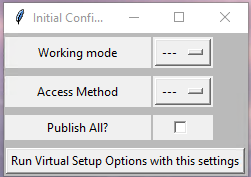
\includegraphics[width=0.6\linewidth]{Im/figures/proposed-work/bios-gui-initial-config}
    \caption{Menu to Select initial configuration for work}\label{fig:proposed-work-bios-gui-initial-config}
  \end{figure}
  
  \begin{figure}[htbp]
    \centering
    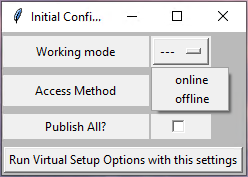
\includegraphics[width=0.6\linewidth]{Im/figures/proposed-work/bios-gui-initial-config-select-mode}
    \caption{Available work mode for the system: Online and Offline}\label{fig:proposed-work-bios-gui-initial-config-select-mode}
  \end{figure}
\end{frame}

\begin{frame}{Setup Knobs Modification: Overview of GUI Actions}
  \begin{table}
    \centering
    \renewcommand{\arraystretch}{1}
%    \caption{Interpretation of buttons on Virtual Setup Page GUI}\label{table:interpretation-of-buttons-in-module}
    \begin{tabular}{p{3cm} | p {7.5cm}}
      Button & Interpretation
      \\ \hline \hline
      Push Changes & Apply changes to system if online mode else apply changes to `bin` file
      \\ \hline View Changes & View saved changes in new window
      \\ \hline Exit & Exit the GUI
      \\ \hline Reload & Reload the GUI
      \\ \hline Discard Changes & Discard any change made, any value if modified are restored to current value
      \\ \hline Load Defaults & Restore to default values and revert any changes made
      \\ \hline
    \end{tabular}
  \end{table}
\end{frame}

\begin{frame}{Setup Knobs Modification: Outcome}
  \begin{itemize}
    \item Cross platform usage
    \item API as a driver in BIOS Firmware
    \item Generic solution for usage types - on \textbf{SUT}, on \textbf{BIOS image}
    \item Information parsing and simulation
    \item Realtime sync for simulation changes
    \item Seamless Integration
  \end{itemize}
\end{frame}

% ========================================================================
% MODULE 2
% ========================================================================
\subsection{Implementation of Parsing}

\begin{frame}{Implementation of Parsing: Format of BIOS Image}
  \begin{figure}[htbp]
    \centering
    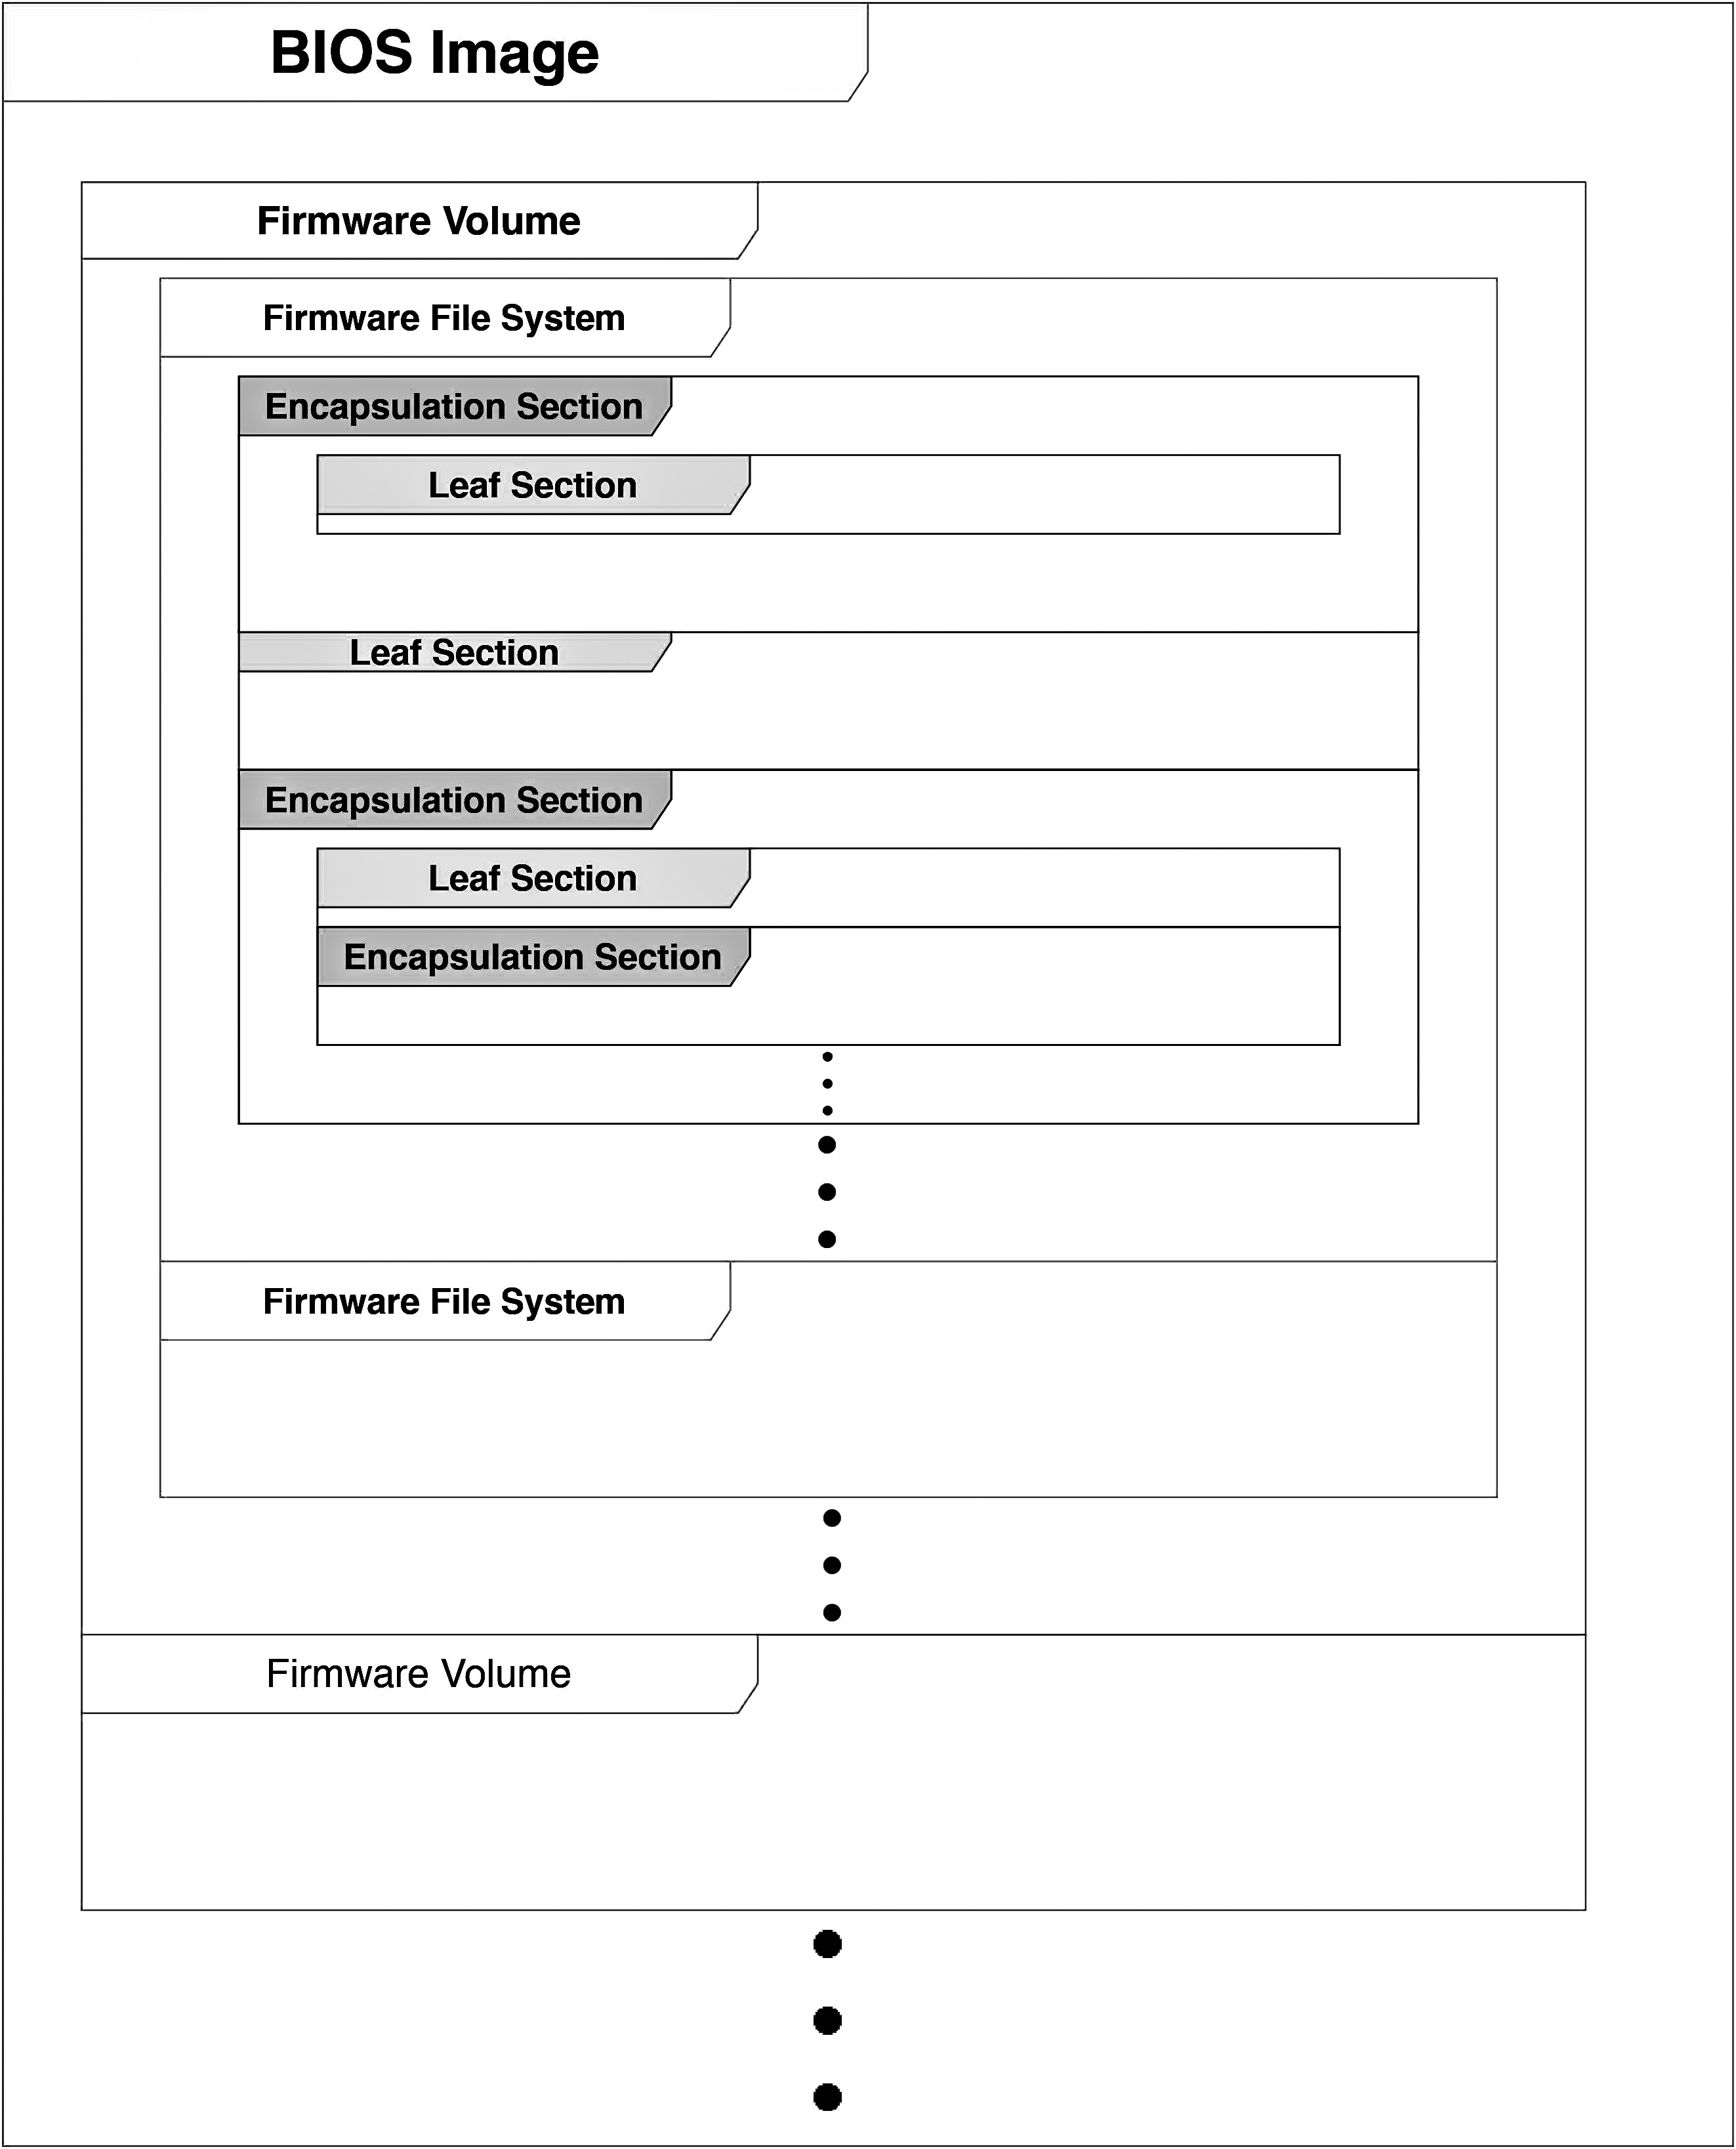
\includegraphics[width=0.5\linewidth]{Im/figures/bios-as-filesystem}
    %		\caption{Each Firmware Volume in BIOS Image}
    %		\label{fig:the-firmware-volume-format}
  \end{figure}
\end{frame}

\begin{frame}{Implementation of Parsing: Work Flow}
  \begin{figure}[htbp]
    \centering
    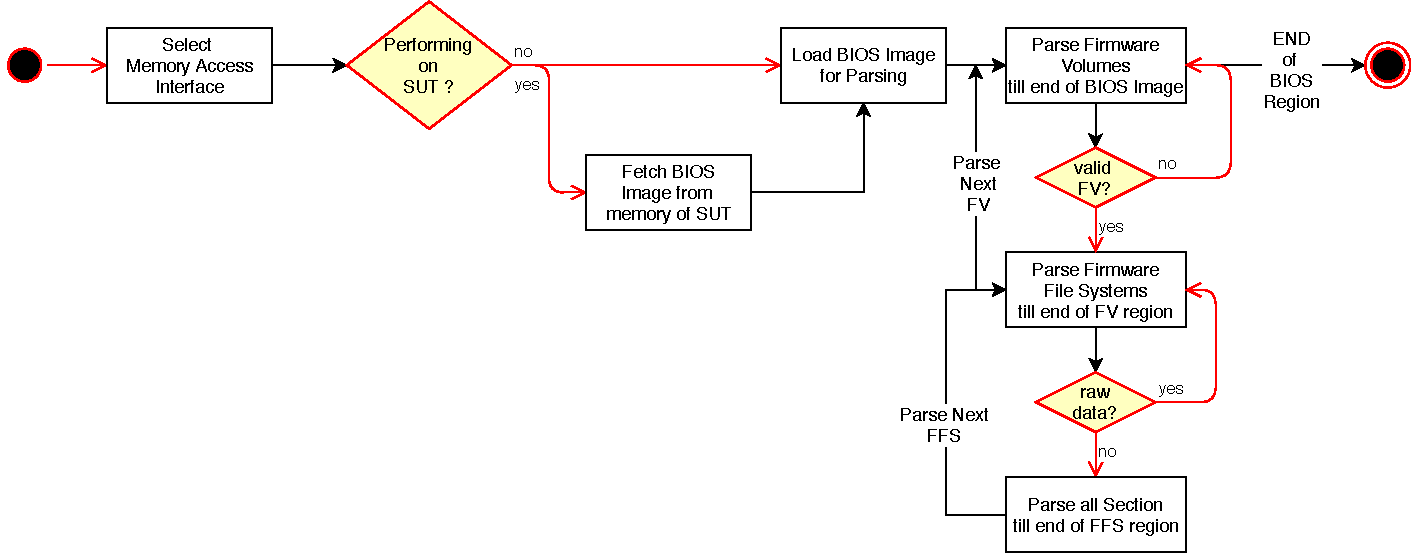
\includegraphics[width=\linewidth]{Im/figures/uefi-parser}
    %    \caption{Each Firmware Volume in BIOS Image}
    %    \label{fig:uefi-parser-flow}
  \end{figure}
\end{frame}

\begin{frame}{Implementation of Parsing: Outcome}
  \begin{itemize}
    \item Human Readable interpretation of BIOS Image
    \item GUIDs Lookup
    \item Verification of existence of module by GUID
    \item Storing the image file system content by GUID
    \item Summarizing changes of two BIOS image
  \end{itemize}
\end{frame}

% ========================================================================
% MODULE 3
% ========================================================================
\subsection{Runtime UEFI Variable Creation}
\begin{frame}{Runtime UEFI Variable Creation: Work Flow}
  \begin{figure}[htbp]
    \centering
    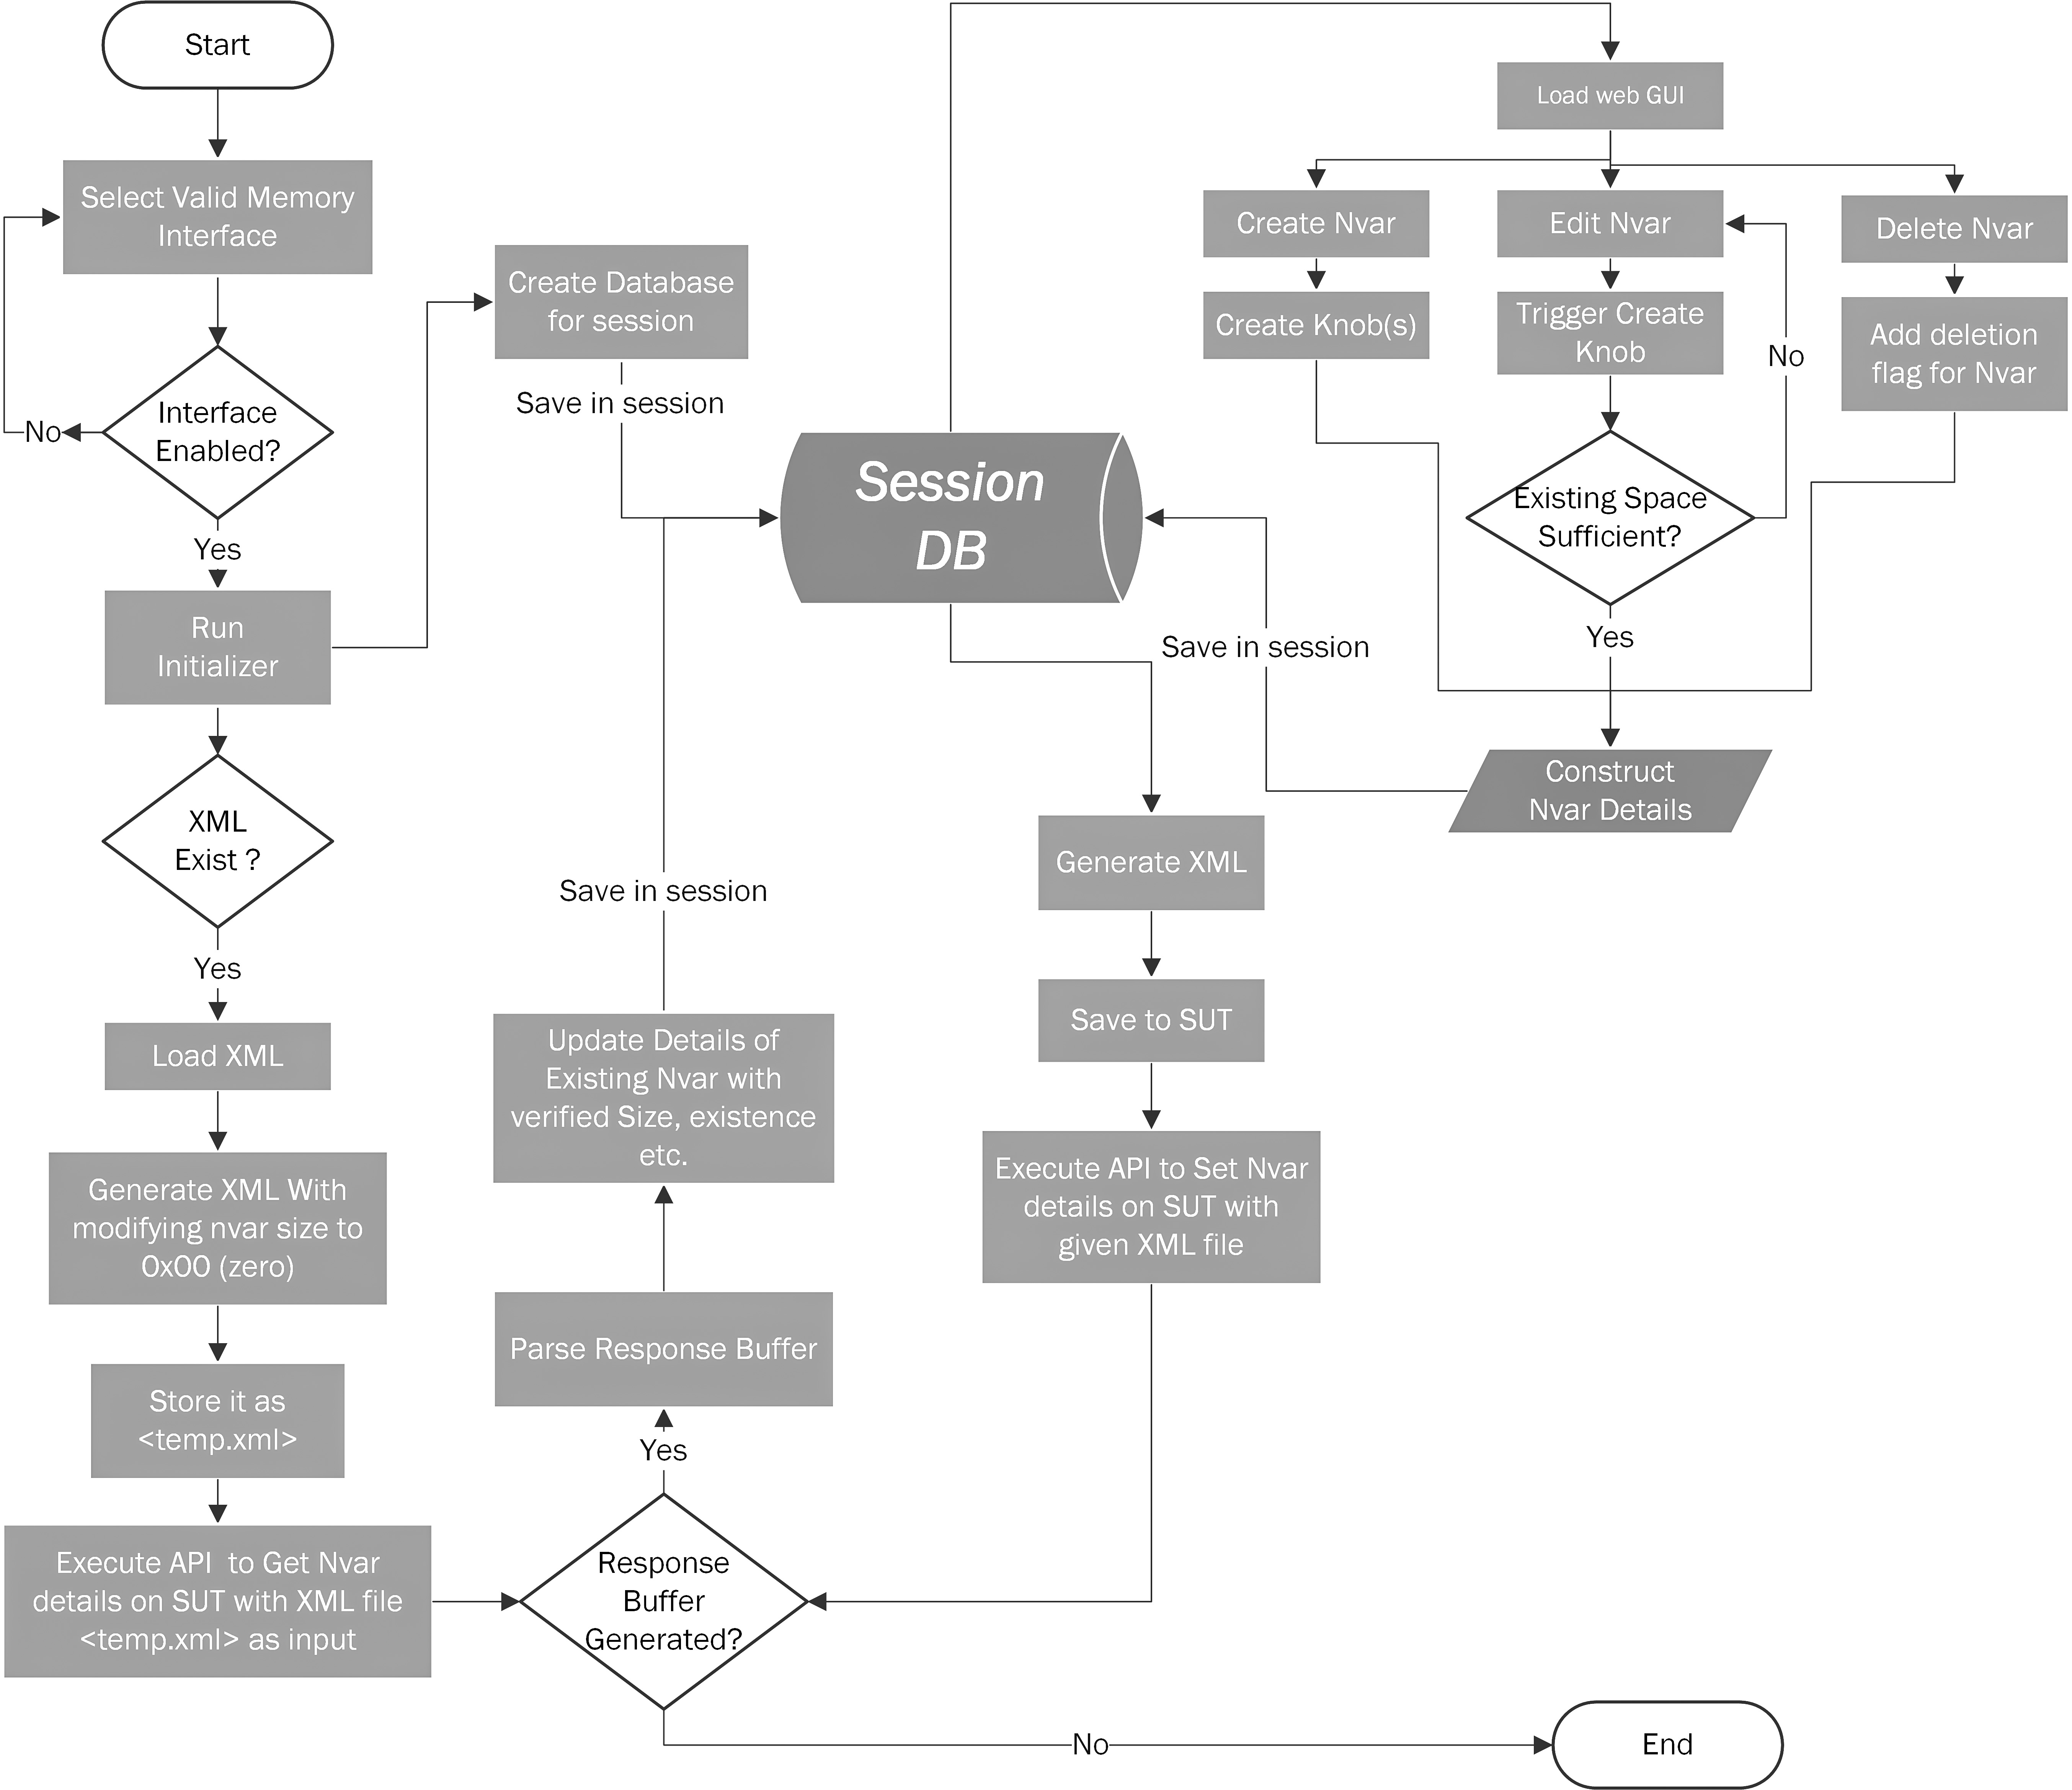
\includegraphics[width=0.6\linewidth]{Im/figures/nvar_web_GUI_flow}
  \end{figure}
\end{frame}


\begin{frame}{Runtime UEFI Variable Creation: Additional Tech Stack}
  \begin{itemize}
    \item Flask
    \item Ajax
    \item jQuery
    \item Javascript
    \item HTML/CSS
    \item XML
    \item JSON
  \end{itemize}
\end{frame}

\begin{frame}[allowframebreaks]{Runtime UEFI Variable Creation: Implementation Snaps}
  \begin{figure}[htbp]
    \centering
    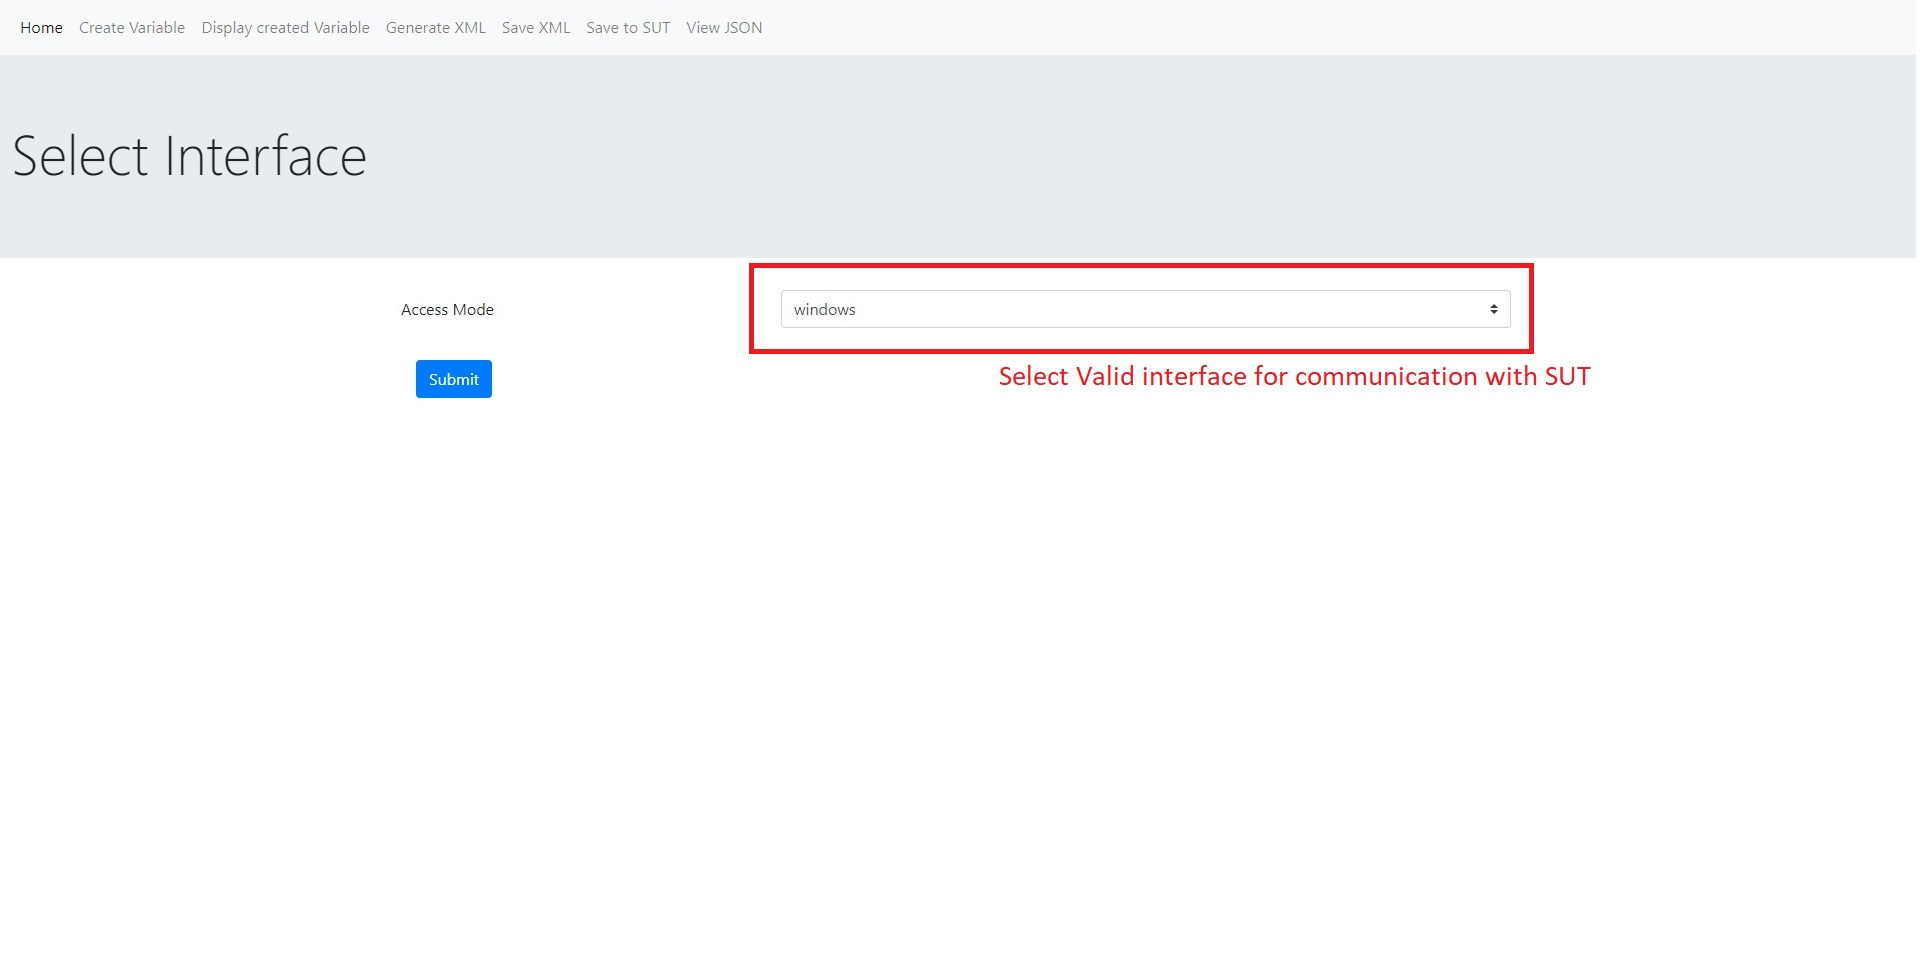
\includegraphics[width=0.9\textwidth]{proposed-work/uefi-variables/home}
    \caption{Home Page to Create UEFI Variable}\label{fig:uefi-variable-home}
  \end{figure}

  \begin{figure}[htbp]
    \centering
    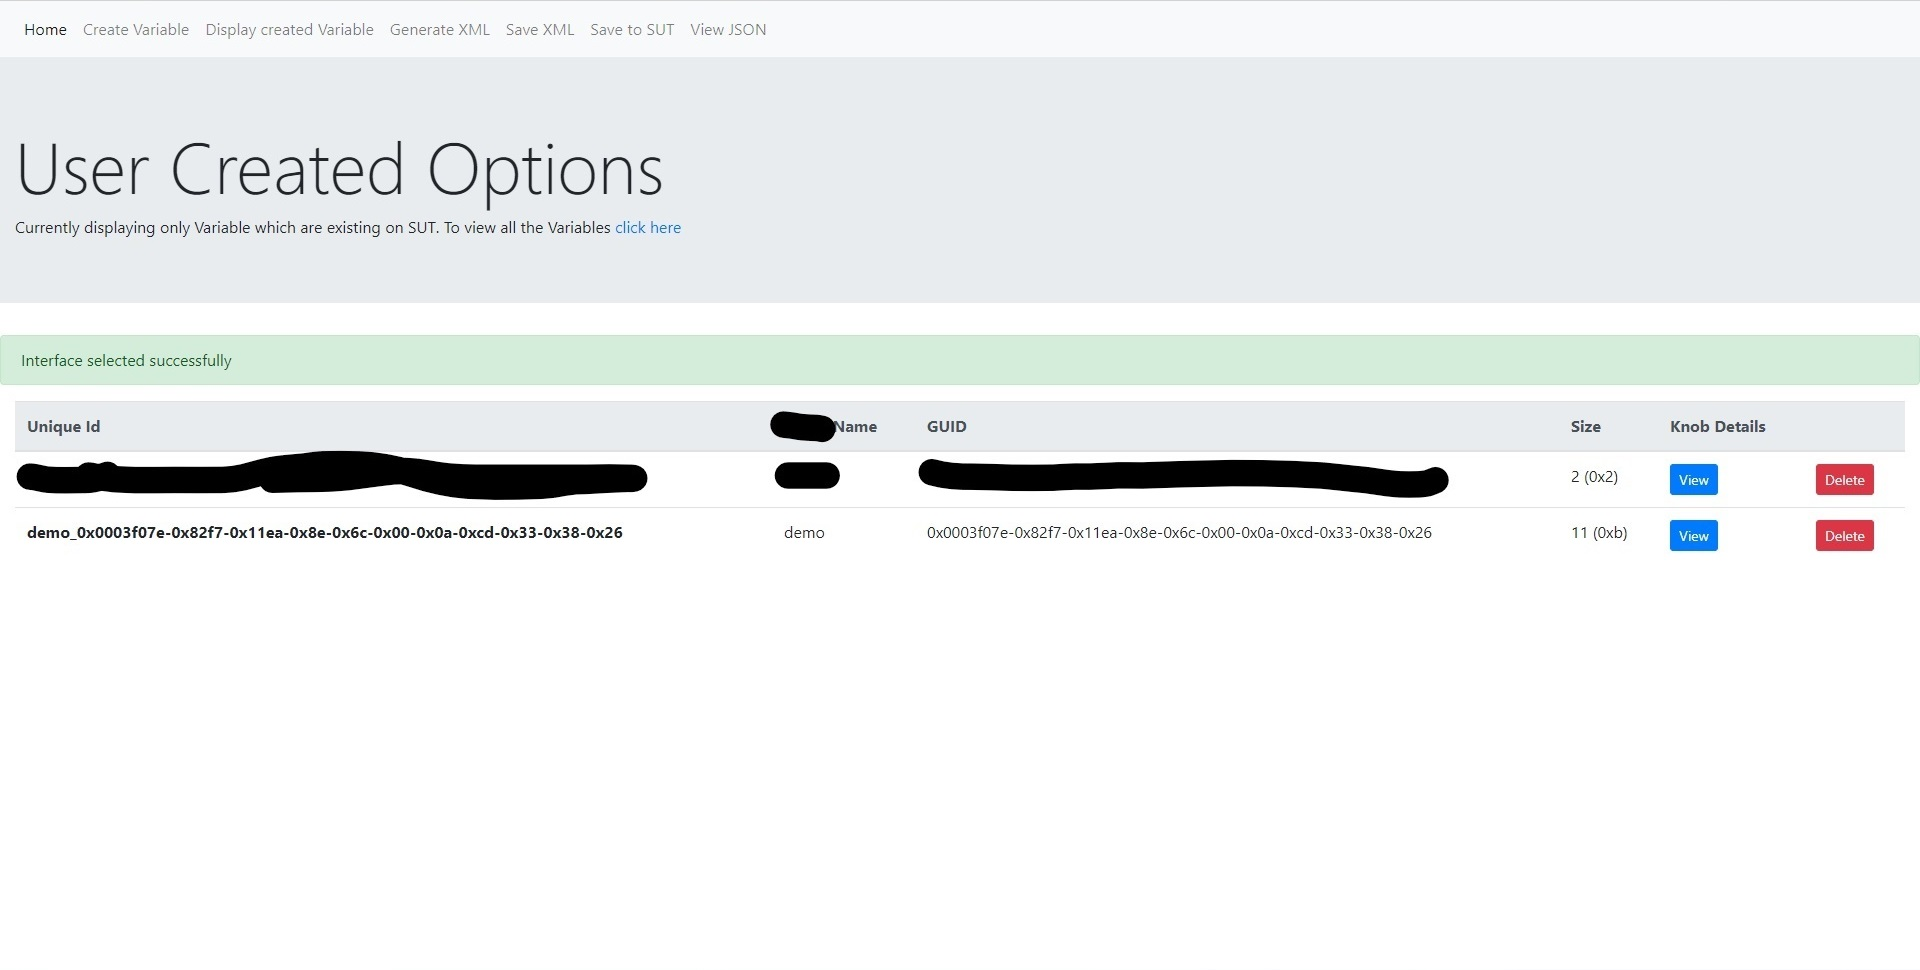
\includegraphics[width=\textwidth]{proposed-work/uefi-variables/created-option}
    \caption{Variables created or exists on SUT}\label{fig:uefi-variable-created-option}
  \end{figure}
  
  \begin{figure}[htbp]
    \centering
    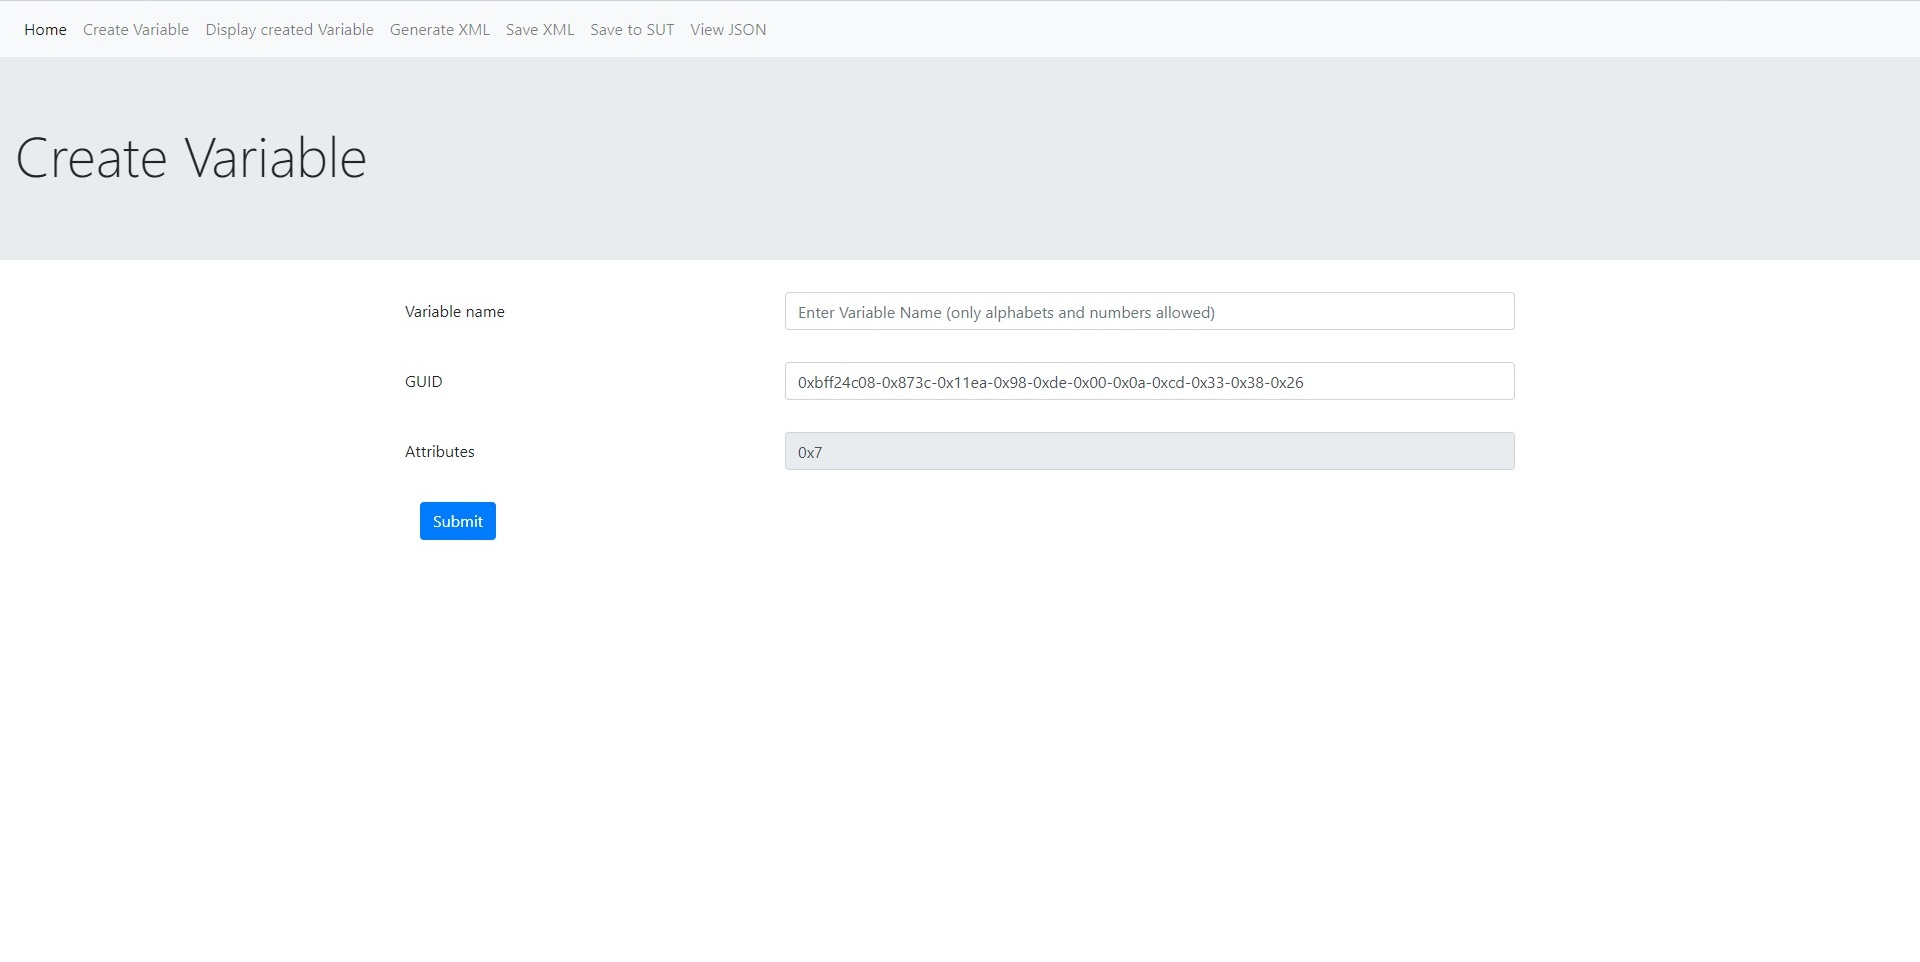
\includegraphics[width=\textwidth]{proposed-work/uefi-variables/create-nvar}
    \caption{Create new UEFI Variable on SUT}\label{fig:uefi-variable-create-nvar}
  \end{figure}
  
  \begin{figure}[htbp]
    \centering
    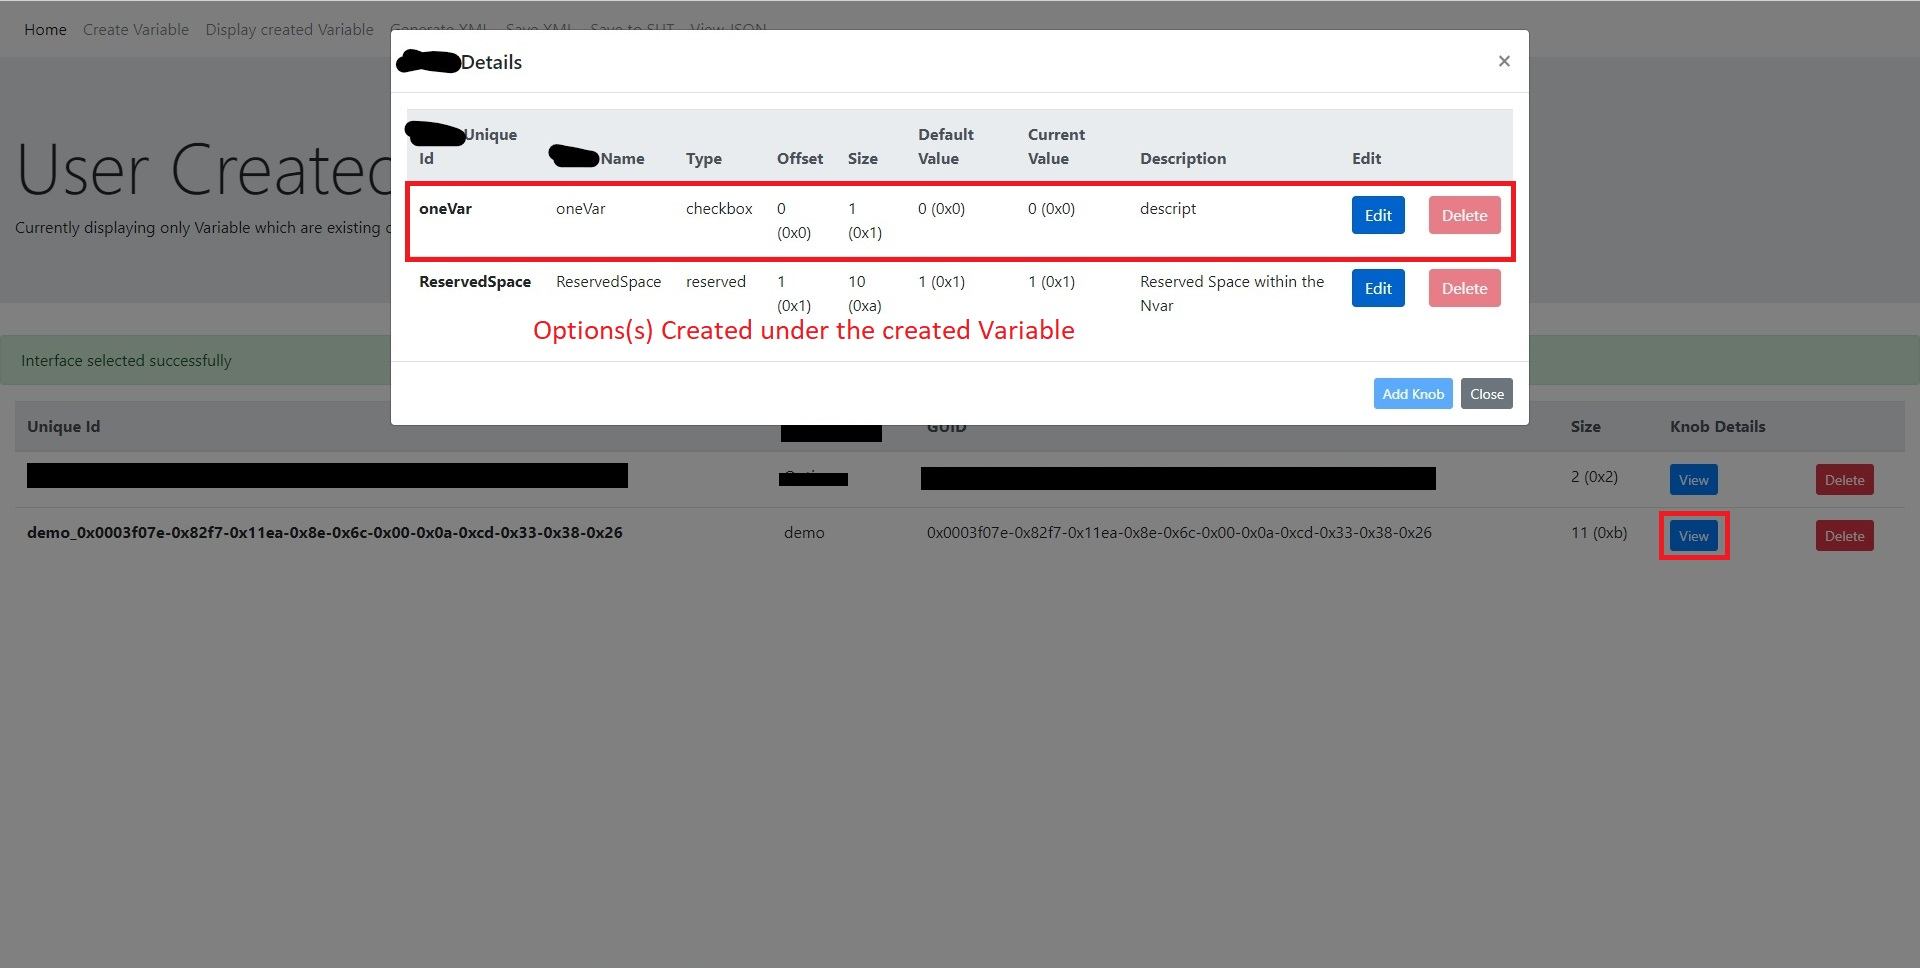
\includegraphics[width=\textwidth]{proposed-work/uefi-variables/var-options}
    \caption{Options listed under Variable}\label{fig:uefi-variable-var-options}
  \end{figure}
  
  \begin{figure}[htbp]
    \centering
    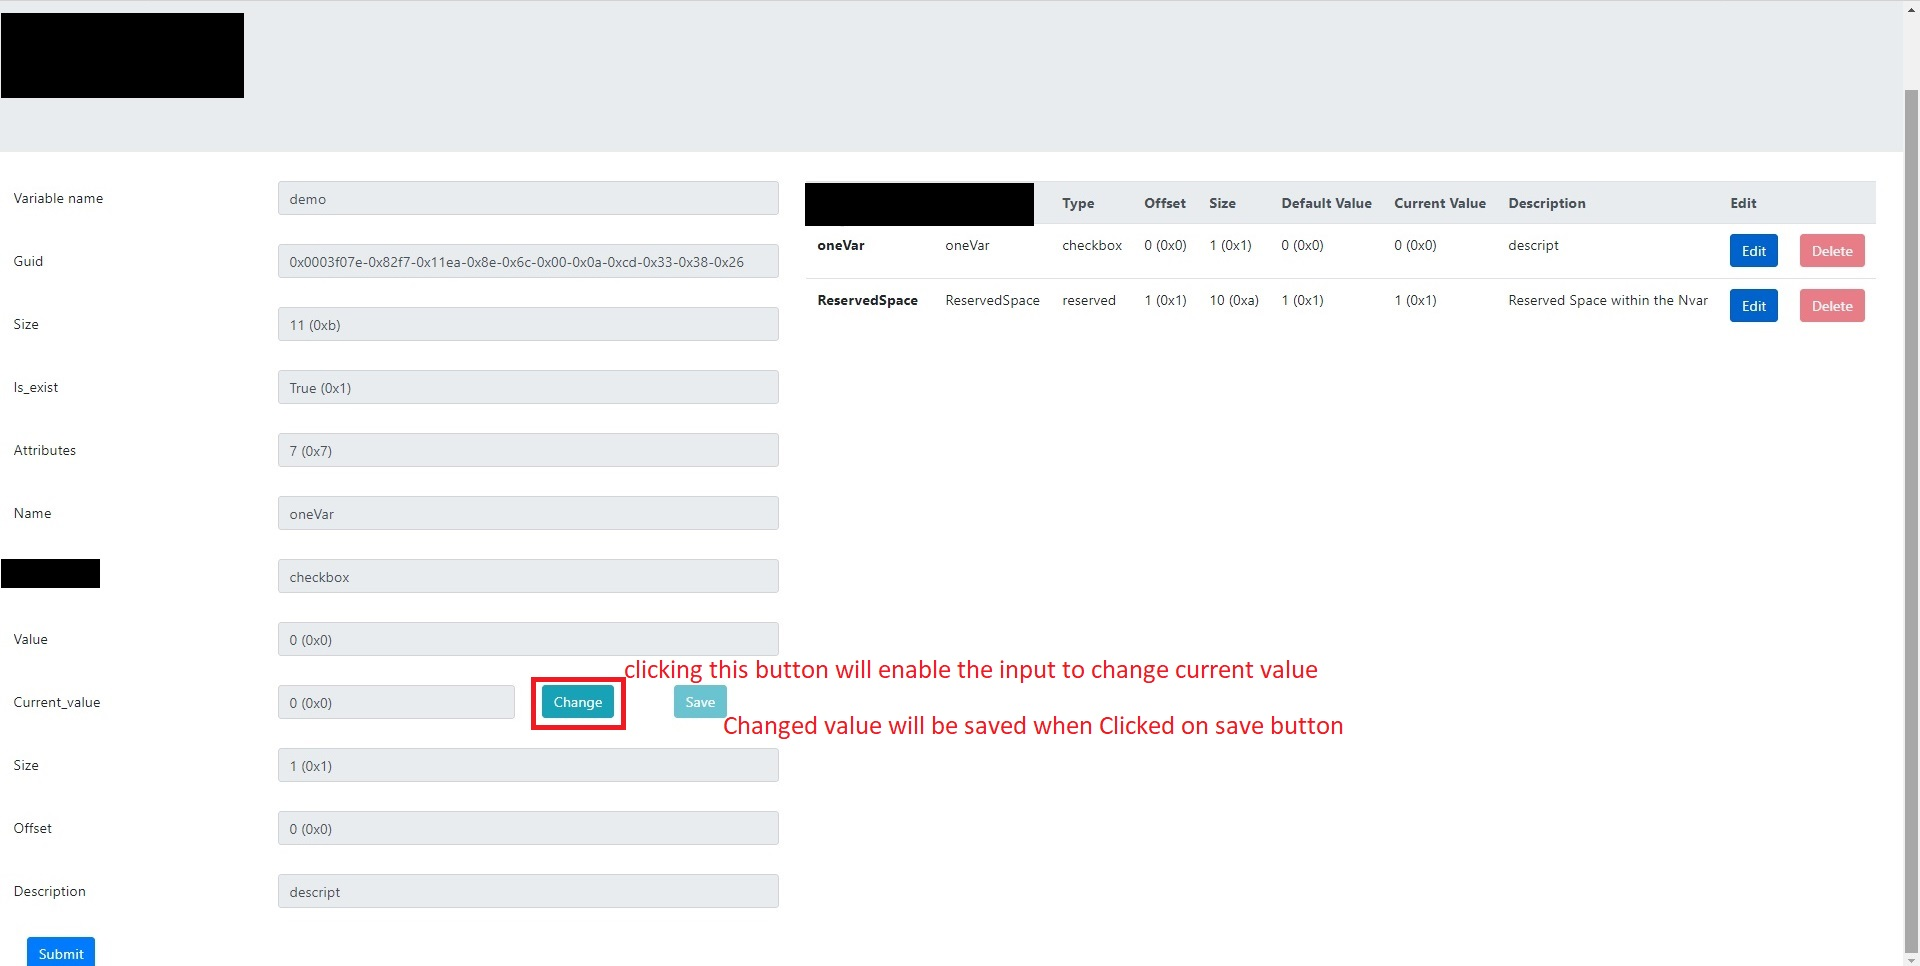
\includegraphics[width=\textwidth]{proposed-work/uefi-variables/edit-option}
    \caption{Edit the Existing Option Created under Variable SUT}\label{fig:uefi-variable-edit-option}
  \end{figure}
  
  \begin{figure}[htbp]
    \centering
    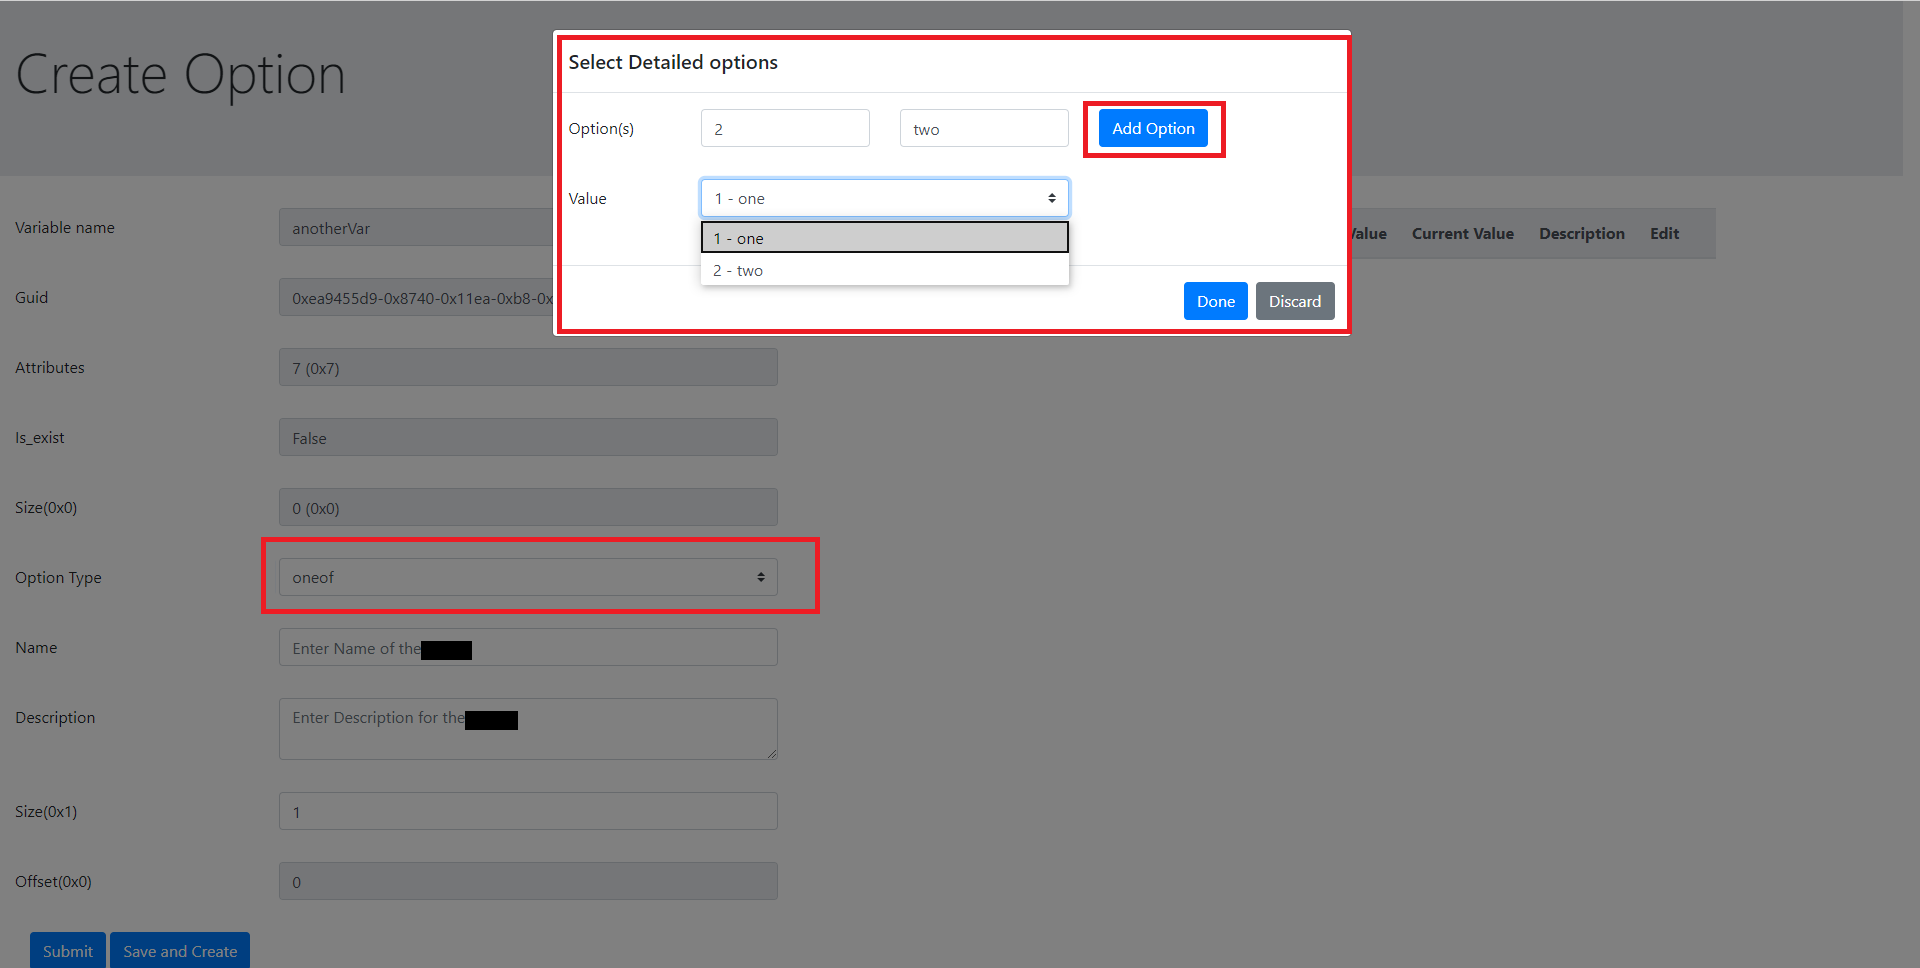
\includegraphics[width=\textwidth]{proposed-work/uefi-variables/add-option}
    \caption{Create New Option(s) under Variable - Oneof Type}\label{fig:uefi-variable-add-option}
  \end{figure}
  
  \begin{figure}[htbp]
    \centering
    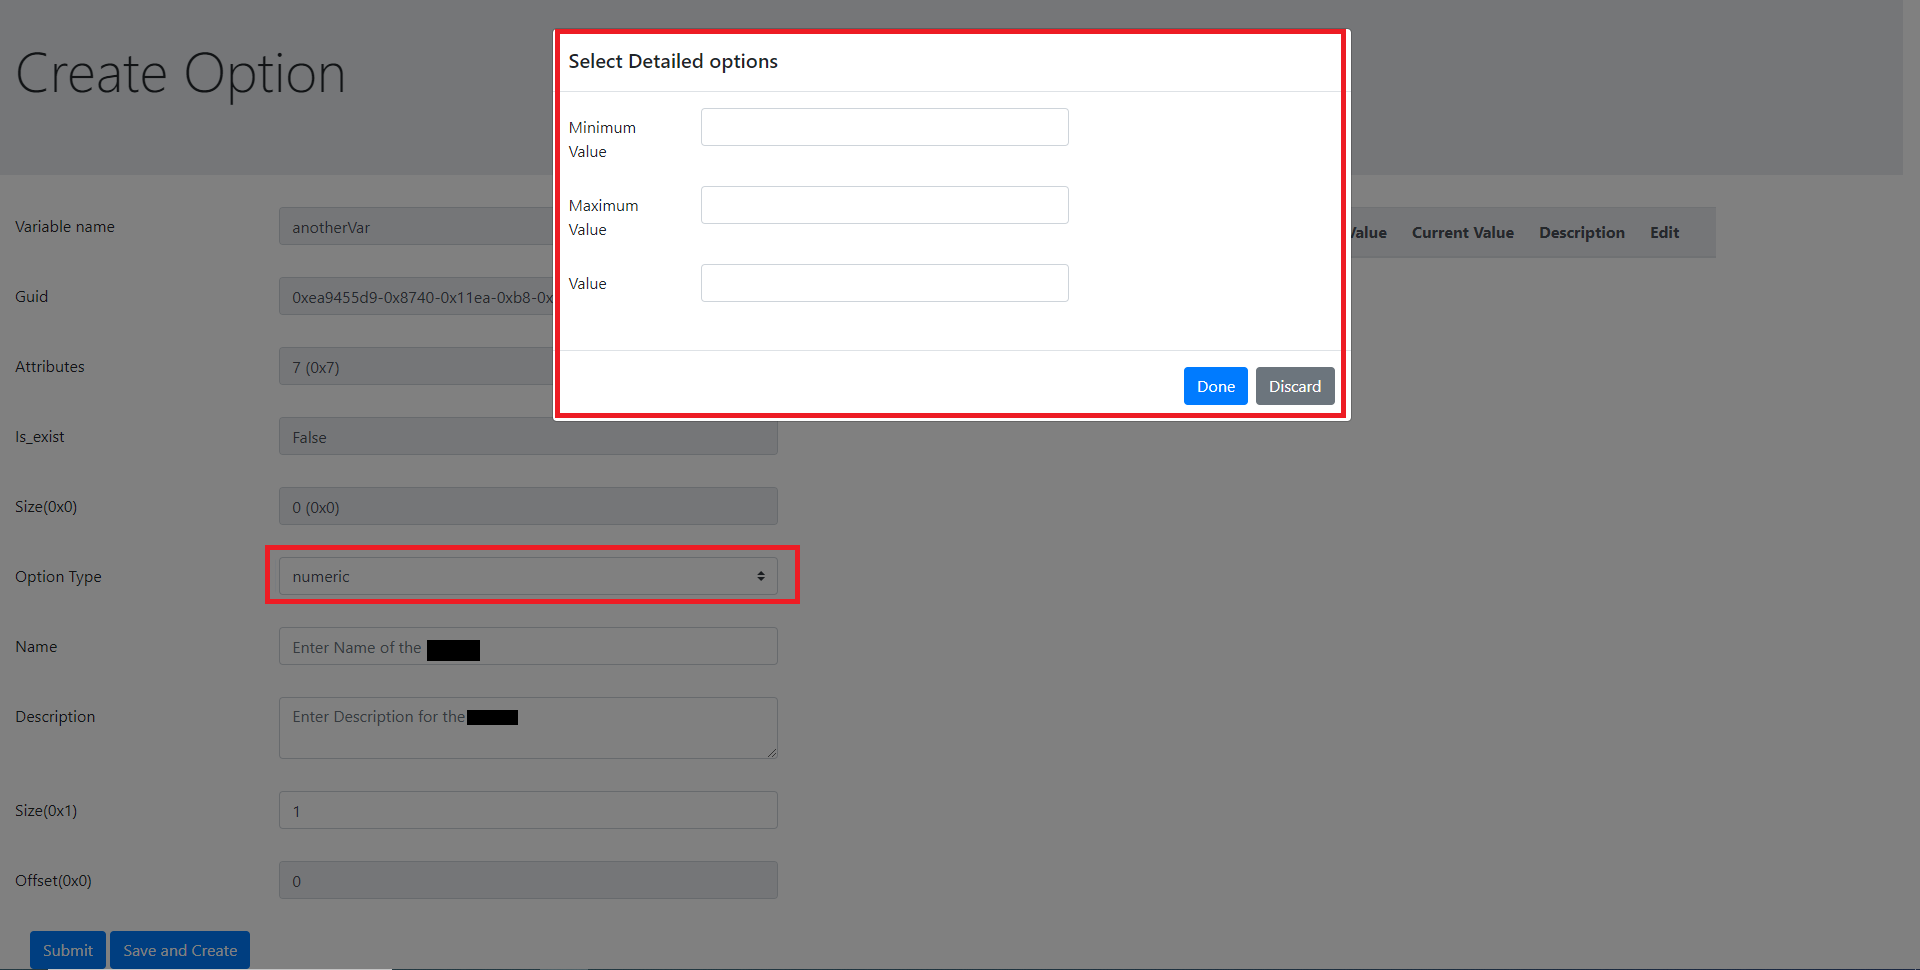
\includegraphics[width=\textwidth]{proposed-work/uefi-variables/numeric}
    \caption{Create New Option(s) under Variable - Numeric Type}\label{fig:uefi-variable-numeric}
  \end{figure}
  
  \begin{figure}[htbp]
    \centering
    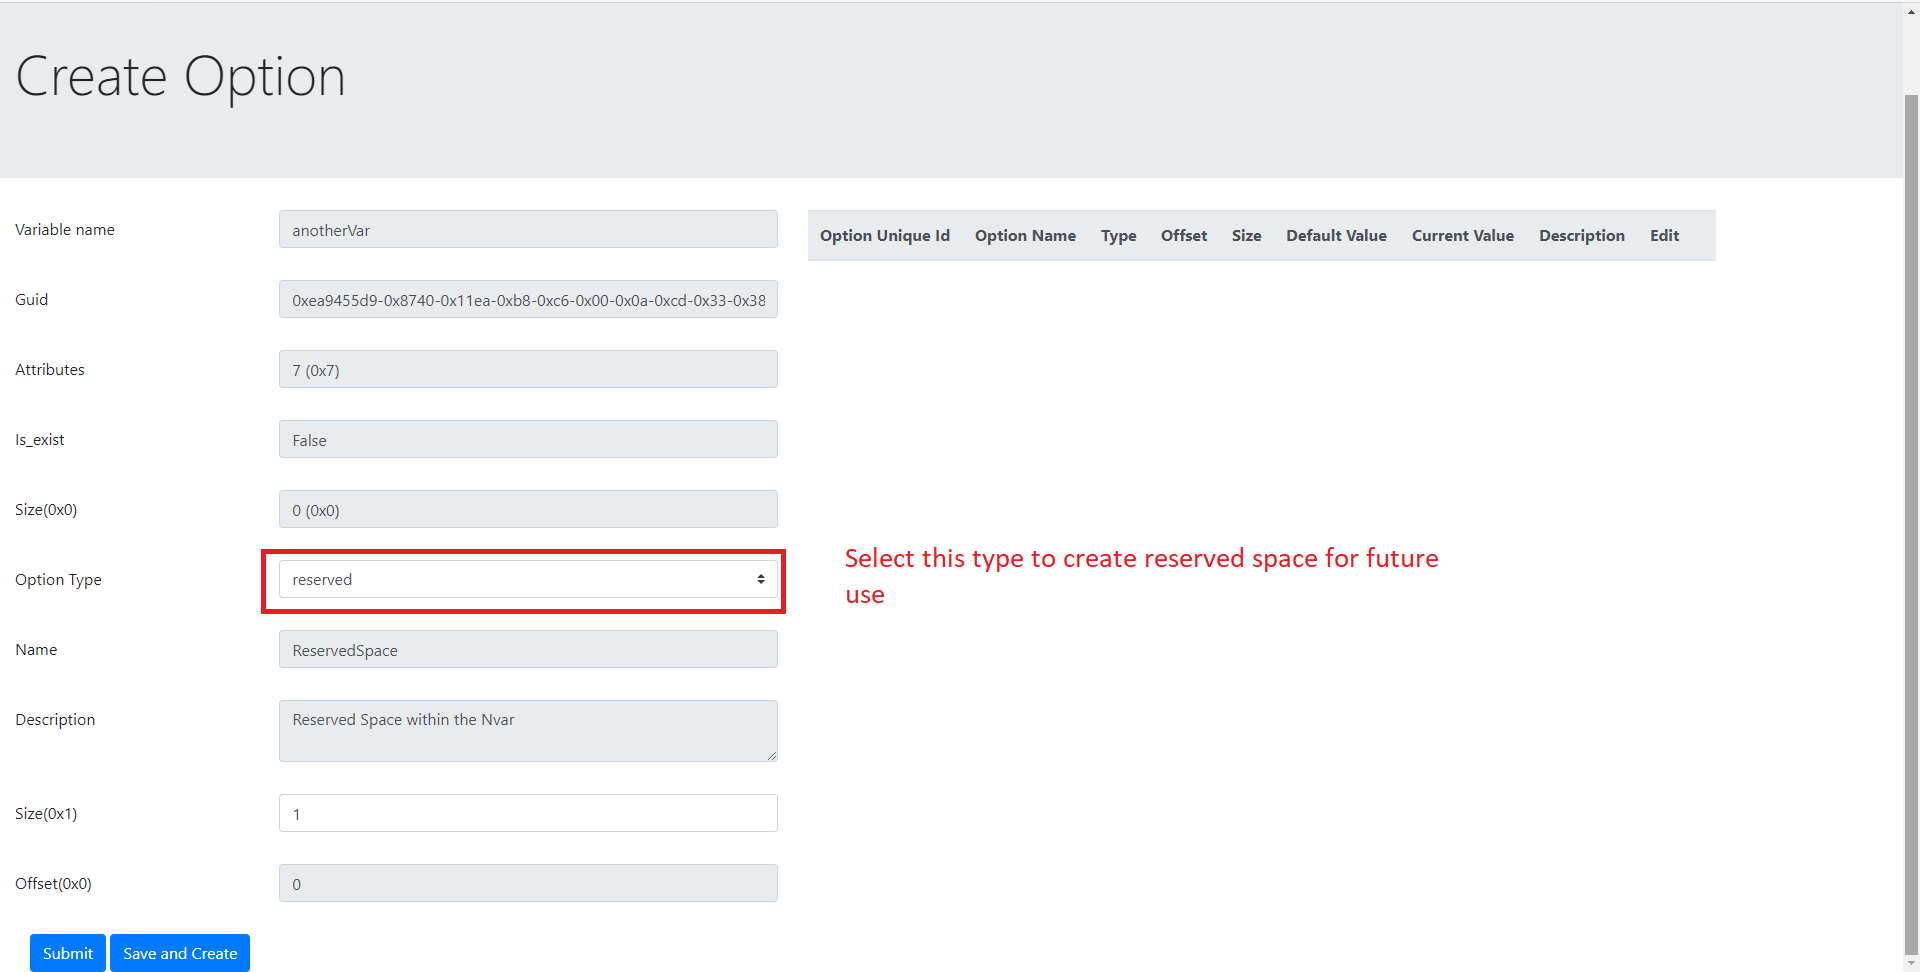
\includegraphics[width=\textwidth]{proposed-work/uefi-variables/reserved-space}
    \caption{Create Reserved Space for future use under Variable}\label{fig:uefi-variable-reserved-space}
  \end{figure}
  
  \begin{figure}[htbp]
    \centering
    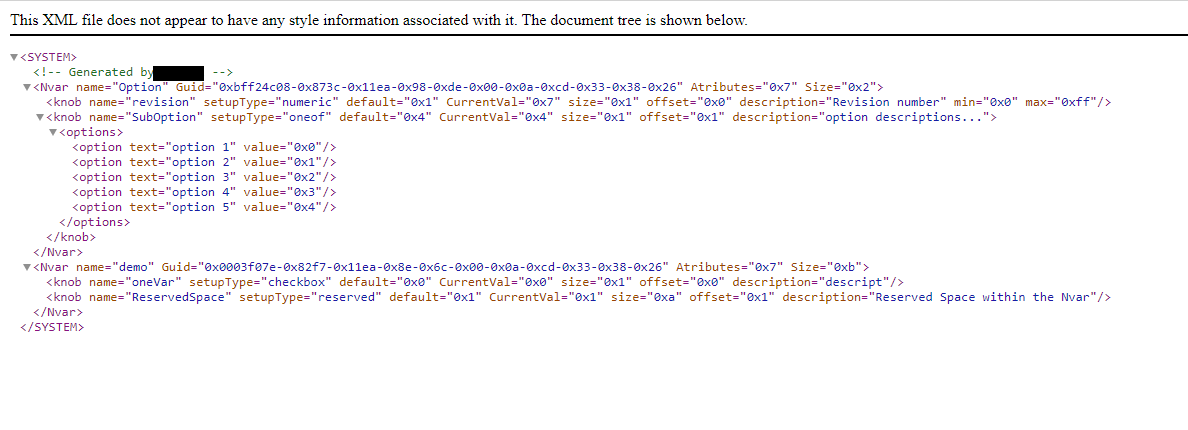
\includegraphics[width=\textwidth]{proposed-work/uefi-variables/generate-xml}
    \caption{Generate XML SUT}\label{fig:uefi-variable-generate-xml}
  \end{figure}

\end{frame}

\begin{frame}{Runtime UEFI Variable Creation: Overview of GUI Actions}
  \begin{table}
    \centering
    \renewcommand{\arraystretch}{1}
%    \caption{Navigation Bar Action}\label{table:navbar-action}
    \begin{tabular}{p{3cm} | p {7.5cm}}
      Button & Interpretation
      \\ \hline \hline
      Create Variable & Opens a form to create new Variable
      \\ \hline Display Created Variable & lists out created variable
      \\ \hline Generate XML & Generate XML from the stored session database
      \\ \hline Save XML & Saves the generated XML on the storage device
      \\ \hline Save to SUT & Applies the Pending changes action (Create/Delete/Modify) to SUT
      \\ \hline View JSON & View the stored session database in the json format
      \\ \hline
    \end{tabular}
  \end{table}
\end{frame}

\begin{frame}{Runtime UEFI Variable Creation: Outcome}
  \begin{itemize}
    \item Avoid providing native BIOS Support
    \item No initial setup overhead
    \item Interactive Web GUI
    \item Quick Modification of Variable
  \end{itemize}
\end{frame}
